\documentclass[11pt]{article}

% ---------------- Packages ----------------
\usepackage[a4paper,margin=1in]{geometry}
\usepackage{amsmath,amssymb,amsfonts}
\usepackage{mathtools}
\usepackage{bm}
\usepackage{booktabs}
\usepackage{array}
\usepackage{longtable}
\usepackage{tabularx}
\usepackage{enumitem}
\usepackage{graphicx}
\usepackage{caption}
\usepackage{subcaption}
\usepackage{float}
\usepackage{pdflscape}
\usepackage{xcolor}
\usepackage[colorlinks=true,linkcolor=blue,citecolor=blue,urlcolor=blue]{hyperref}
\usepackage[activate={true,nocompatibility},final,tracking=true,kerning=true,spacing=true,factor=1100,stretch=10,shrink=10,expansion=false,protrusion=true]{microtype}
\usepackage{setspace}
\usepackage{titlesec}
\usepackage{fancyhdr}
\usepackage{parskip}
\usepackage{url}
\usepackage{xspace}
\usepackage{authblk}
\usepackage[numbers,sort&compress]{natbib}
\usepackage{tikz}
\usetikzlibrary{arrows.meta,positioning,fit,backgrounds,calc,shapes.geometric}

\emergencystretch=3em
\graphicspath{{figures_v4/}}
\setlist[itemize]{leftmargin=1.6em,itemsep=0.25em,topsep=0.35em}
\setlist[enumerate]{leftmargin=1.6em,itemsep=0.25em,topsep=0.35em}
\titleformat{\section}{\Large\bfseries}{\thesection}{0.8em}{}
\titleformat{\subsection}{\large\bfseries}{\thesubsection}{0.8em}{}
\titleformat{\subsubsection}{\normalsize\bfseries\itshape}{\thesubsubsection}{0.6em}{}

\pagestyle{fancy}
\fancyhf{}
\fancyhead[L]{\small RRRM-2 v6 methods compendium}
\fancyhead[R]{\small \thepage}
\renewcommand{\headrulewidth}{0.4pt}

\newcommand{\code}[1]{\texttt{#1}}
\newcommand{\pkg}[1]{\textsf{#1}}
\newcommand{\gene}[1]{\textit{#1}}
\newcommand{\RRRM}{RRRM-2\xspace}
\newcommand{\ISS}{ISS-T\xspace}
\newcommand{\LAR}{LAR\xspace}
\newcommand{\OSD}{OSDR\xspace}
\newcommand{\FDR}{FDR\xspace}

\definecolor{stageblue}{RGB}{216,231,247}
\definecolor{stagegreen}{RGB}{216,239,228}
\definecolor{stagegold}{RGB}{250,235,197}
\definecolor{stagerose}{RGB}{246,220,220}
\definecolor{stageviolet}{RGB}{228,220,245}
\definecolor{stagegray}{RGB}{235,235,235}
\definecolor{ink}{RGB}{40,45,55}
\definecolor{muted}{RGB}{95,100,115}

\title{\textbf{Methods}\\[0.35em]
\large A v6 methods compendium for the RRRM-2 kidney spaceflight transcriptome analysis}
\author{Ibrahim Shahid}
\affil{Independent research draft for mentor feedback\\Authorship/collaboration structure pending}
\date{Draft v6 methods compendium, May 2026}

\begin{document}
\maketitle

\begin{abstract}
\noindent
This document formalizes the analysis pipeline used to produce the v6 RRRM-2 kidney transcriptome results. It is written as a companion to the results-only PDF. The goal is not only to state statistical procedures, but to make the whole analysis intelligible: what each method consumes, what it computes, what it produces, and which biological claim it supports. The core pipeline starts with residualized kidney expression, scores biologically interpretable feature layers, tests whether the original RRRM-2 age-rewiring contrast is stable, redirects the main inference toward cross-OSDR flight-vector recurrence, builds an ISS-T/OSD-513 recurrent remodeling axis, decomposes that axis into a matrix-high / DCT-low tubulointerstitial state, evaluates live-return attenuation/divergence, uses OSD-253 as TLR4/innate context rather than strict validation, and keeps WGCNA plus LIONESS/node2vec as structural annotation and exploratory gene-prioritization layers.
\end{abstract}

\vspace{0.5em}
\noindent\textbf{Companion artifact.} This document is intended to sit beside \path{latex_paper/results.pdf}. The results PDF reports what was found; this methods PDF explains how each result was made and how the analysis pieces fit together.

\clearpage
\tableofcontents
\clearpage

% =====================================================================
\section{What the Pipeline Is Trying To Do}

\subsection{The conceptual problem}

The project began as a high-dimensional network-rewiring analysis of RRRM-2 kidney RNA-seq. RRRM-2 is attractive because it crosses age, mission arm, and flight environment in the same study. That design naturally suggests a question like: does spaceflight change the way kidney aging biology is coordinated, and does that differ between terminal dissection and live animal return?

The later v6 analysis keeps that question visible, but it does not force the data to support it. The reason is simple: the within-arm control-aging vector is estimated from only five young ground-control and five old ground-control mice per arm. That is a very small basis for a high-dimensional age-direction claim. Therefore, the pipeline first asks whether the original age-rewiring direction is stable enough to be a claim. It is not stable at the primary module/pathway scale. That negative result becomes a guardrail.

The strongest surviving question is different:

\begin{quote}
Does RRRM-2 identify an arm-specific kidney flight-remodeling direction that recurs in independent OSDR kidney spaceflight data, and what biology defines that direction?
\end{quote}

The pipeline is therefore organized around a claim hierarchy rather than around one favorite method. The methods are used as layers of evidence:

\begin{itemize}
  \item Stability tests decide whether the original age-rewiring claim is supportable.
  \item Cross-OSDR contrast vectors test whether the RRRM-2 ISS-T flight direction recurs outside RRRM-2.
  \item A recurrent remodeling axis turns cross-cohort agreement into a sample-level score.
  \item Mechanism and state-space scoring translate the axis into kidney biology.
  \item LAR attenuation/divergence analysis tests whether live return repeats, attenuates, reverses, or redirects the ISS-T state.
  \item OSD-253 asks whether TLR4/innate biology is associated with, or required for, the remodeling state.
  \item WGCNA, LIONESS, and node2vec annotate modules and prioritize genes inside the pathway-level program.
\end{itemize}

\subsection{The main data-to-claim chain}

The central chain of evidence is:

\begin{center}
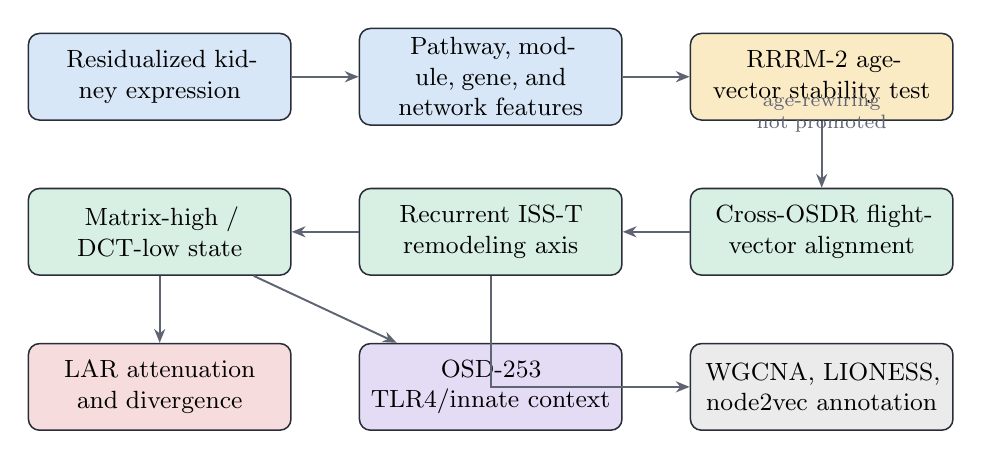
\begin{tikzpicture}[
  node distance=0.85cm and 0.85cm,
  box/.style={rectangle, rounded corners=4pt, draw=ink, line width=0.55pt,
    align=center, text width=3.1cm, minimum height=1.1cm, font=\small},
  arrow/.style={-{Stealth[length=5pt,width=4pt]}, line width=0.7pt, draw=muted},
  note/.style={font=\scriptsize, align=center, text=muted, text width=3.1cm}
]
\node[box, fill=stageblue] (expr) {Residualized kidney expression};
\node[box, fill=stageblue, right=of expr] (features) {Pathway, module, gene, and network features};
\node[box, fill=stagegold, right=of features] (stability) {RRRM-2 age-vector stability test};
\node[box, fill=stagegreen, below=of stability] (cross) {Cross-OSDR flight-vector alignment};
\node[box, fill=stagegreen, left=of cross] (axis) {Recurrent ISS-T remodeling axis};
\node[box, fill=stagegreen, left=of axis] (state) {Matrix-high / DCT-low state};
\node[box, fill=stagerose, below=of state] (lar) {LAR attenuation and divergence};
\node[box, fill=stageviolet, right=of lar] (osd253) {OSD-253 TLR4/innate context};
\node[box, fill=stagegray, right=of osd253] (gene) {WGCNA, LIONESS, node2vec annotation};

\draw[arrow] (expr) -- (features);
\draw[arrow] (features) -- (stability);
\draw[arrow] (stability) -- node[note, above, yshift=0.15cm]{age-rewiring not promoted} (cross);
\draw[arrow] (cross) -- (axis);
\draw[arrow] (axis) -- (state);
\draw[arrow] (state) -- (lar);
\draw[arrow] (state) -- (osd253);
\draw[arrow] (axis) |- (gene);

\end{tikzpicture}
\end{center}

The project is therefore best described as a cross-cohort remodeling-state analysis with exploratory network annotation.

% =====================================================================
\section{Pipeline Overview}

\subsection{Method-to-result crosswalk}

\begin{landscape}
\small
\setlength{\tabcolsep}{4pt}
\begin{longtable}{p{0.17\linewidth}p{0.20\linewidth}p{0.25\linewidth}p{0.27\linewidth}}
\caption{How each method contributes to the v6 results.}\\
\toprule
Method & Main input & Main output & Result or interpretation supported \\
\midrule
\endfirsthead
\toprule
Method & Main input & Main output & Result or interpretation supported \\
\midrule
\endhead
Expression preprocessing and residualization & RRRM-2 expression matrix, metadata, deconvolution covariates & Residualized expression matrix and matched sample metadata & Reduces technical and cell-composition confounding before pathway, module, and network analyses. \\
Feature scoring & Residualized expression and curated gene sets/modules & Pathway scores, mechanism scores, module eigengenes, gene-level features & Provides interpretable analysis layers: ECM, fibrosis, DCT/NCC-WNK transport, inflammation, S1P, clock, WGCNA modules, and gene summaries. \\
Control-aging vector stability & Young and old GC samples within each arm & Bootstrap cosine stability table & Shows RRRM-2 cannot support the original within-cohort age-rewiring claim at primary pathway/module scale. \\
Cross-OSDR flight-vector alignment & RRRM-2 arm-specific pathway vectors plus OSD-513 and OSD-253 pathway vectors & Cosines, bootstrap intervals, permutation sensitivities & Establishes the main positive result: RRRM-2 ISS-T aligns with OSD-513; LAR is directionally opposite but not confirmatory under the permutation null. \\
Recurrent remodeling-axis construction & Concordant RRRM-2 ISS-T and OSD-513 pathway effects & Axis weights and sample remodeling scores & Converts cross-cohort agreement into a scalar remodeling score oriented as ECM/fibrosis high and DCT transport low. \\
Tubulointerstitial state-space & Mechanism scores and recurrent-axis components & Matrix component, DCT component, matrix-minus-DCT scalar & Makes the biology legible as a matrix-high / DCT-low state rather than an abstract vector. \\
Deconvolution overlay & State scores plus cell-type deconvolution estimates & Spearman correlations between state components and estimated proportions & Tests whether the state is simply explained by estimated DCT or fibroblast fraction; v6 finds little evidence for that. \\
LAR attenuation/divergence framework & ISS-T and LAR FLT-minus-GC vectors across feature layers & Cosines, projections, component interactions, model calls & Distinguishes pooled attenuation from confirmed reversal; supports mechanism-level divergence more than state-level reversal. \\
OSD-253 TLR4 discriminator & C57BL/6J and C3H/HeJ flight/control contrasts under two control definitions & Strain-specific effects and strain deltas & Supports TLR4/innate association, not strict TLR4 requirement. \\
WGCNA & Residualized expression and module eigengene models & Modules, eigengenes, hub genes, preservation summaries & Provides structural annotation of ECM/cell-migration and multi-module remodeling programs. \\
LIONESS & Shared network skeleton and sample expression & Sample-specific networks and node-strength summaries & Supports exploratory sample-specific network and gene-neighborhood annotation. \\
node2vec plus Procrustes & Predicted condition networks and configured anchors & Aligned graph embeddings and local-neighborhood displacement & Provides exploratory gene-priority information about local network movement. \\
Gene-priority composite & node2vec displacement, LIONESS node strength, OSD-513 support, expression effect & Ranked candidate genes and enrichment sensitivity tables & Nominates follow-up genes without turning them into primary discovery claims. \\
External aging-axis projection & Tabula Muris Senis kidney aging vector and RRRM-2 arm vectors & Projection coefficients and residual summaries & Argues the ISS-T signal is remodeling/transport biology rather than simple accelerated aging. \\
\bottomrule
\end{longtable}
\normalsize
\end{landscape}

\subsection{Output-to-method map}

\begin{longtable}{p{0.31\textwidth}p{0.28\textwidth}p{0.32\textwidth}}
\caption{Primary output files and the methods that generate them.}\\
\toprule
Output & Producing method & Used for \\
\midrule
\endfirsthead
\toprule
Output & Producing method & Used for \\
\midrule
\endhead
\path{contrast_vectors/agc_stability_report.tsv} & Control-aging vector stability & Table of original age-rewiring stability. \\
\path{contrast_vectors/cross_osdr_recurrence/cross_osdr_alignment_summary.tsv} & Cross-OSDR flight-vector recurrence & ISS-T/OSD-513 recurrence and LAR anti-alignment summary. \\
\path{mechanism_axis/recurrent_axis_weights.tsv} & Recurrent remodeling-axis construction & Axis-defining pathway effects and weights. \\
\path{mechanism_axis/sample_remodeling_scores.tsv} & Recurrent remodeling-axis scoring & Mouse-level remodeling scores used in main figures. \\
\path{mechanism_axis/mechanism_score_associations.tsv} & Mechanism scoring and Spearman association & Mechanism heatmap and biology interpretation. \\
\path{tubulointerstitial_state/state_space_group_effects.tsv} & State-space component scoring & Matrix/DCT component effect figure and text. \\
\path{tubulointerstitial_state/state_space_component_correlations.tsv} & Deconvolution overlay & Tests whether state components track estimated cell proportions. \\
\path{tubulointerstitial_state/targeted_renal_gene_panel.tsv} & Targeted residualized-expression extraction & Renal gene heatmap. \\
\path{lar_reversal/lar_reversal_vector_summary.tsv} & LAR vector comparison & Attenuation/reversal/divergence model calls. \\
\path{lar_reversal/lar_reversal_component_effects.tsv} & LAR component effects & Age-pooled and age-stratified component effects. \\
\path{lar_reversal/lar_reversal_pathway_interactions.tsv} & Arm-by-flight interactions & Interaction evidence for matrix, S1P, clock, and transport features. \\
\path{lar_reversal/lar_mechanism_switch_scores.tsv} & Descriptive mechanism-axis projection & Hypothesis-generating mechanism sketches, not confirmatory tests. \\
\path{mechanism_axis/osd253_tlr4_discriminator.tsv} & OSD-253 strain/context analysis & TLR4-associated versus TLR4-required interpretation. \\
\path{external_aging_axis/*/tms_projection_*.tsv} & External aging-axis projection & Distinguishes remodeling from simple aging mimicry. \\
\path{mechanism_axis/gene_axis_priority_top25.tsv} & LIONESS/node2vec gene prioritization & Candidate gene list for exploratory follow-up. \\
\bottomrule
\end{longtable}

% =====================================================================
\section{Datasets and Metadata Logic}

\subsection{RRRM-2 / OSD-771}

RRRM-2, also identified as OSD-771, is the discovery and factorial bridge cohort. It contains female C57BL/6NTac mouse kidney RNA-seq samples crossing:

\begin{itemize}
  \item Age: young and old.
  \item Mission arm: ISS terminal dissection (ISS-T) and live animal return (LAR).
  \item Environment group: flight (FLT), habitat ground control (GC), vivarium control (VIV), and basal/pre-flight (BSL).
\end{itemize}

The key design feature is that each Age $\times$ Arm $\times$ Environment cell contains five biological replicates. This makes the design unusually clean for rodent spaceflight transcriptomics, but it also makes high-dimensional interaction and age-vector estimation fragile. The pipeline therefore treats RRRM-2 as a bridge cohort: it defines arm-specific flight directions and lets those directions be tested against external cohorts.

The primary RRRM-2 flight contrasts are FLT minus habitat GC within arm and, when relevant, within age. VIV and BSL samples are retained for preprocessing and metadata context, but they are not pooled into the primary flight-versus-habitat-control contrast vectors.

\subsection{OSD-513}

OSD-513 is the main external recurrence cohort. It contributes an independent kidney flight-minus-ground vector with a larger powered FLT/GC comparison than each RRRM-2 arm-age cell. It differs from RRRM-2 in metadata and mission context, so it is not pooled at raw-expression level. Instead, it is compared at the level of pathway vectors.

This matters because the recurrence question is directional:

\begin{quote}
Do the same kidney pathway features move in the same direction in RRRM-2 ISS-T and OSD-513?
\end{quote}

The answer is the core positive result of v6.

\subsection{OSD-253}

OSD-253 is not treated as a clean recurrence cohort. It is a mechanism-context cohort because it includes C57BL/6J and C3H/HeJ mice. C3H/HeJ is useful because it has impaired TLR4 signaling, which creates a natural check on whether the remodeling state is strictly TLR4-dependent.

OSD-253 has control-definition complexity. The original GC scenario is closer to the original sequencing/control context but has light-history concerns. The white-LED rerun control scenario improves the light comparison but introduces read-length and library comparability concerns. The pipeline therefore runs both scenarios and interprets OSD-253 as context, not as single-endpoint validation.

\subsection{Tabula Muris Senis kidney aging reference}

The Tabula Muris Senis kidney reference provides an external aging direction. The RRRM-2 internal age direction is small-sample and unstable, so the external reference asks a simpler question: does the ISS-T flight-remodeling vector project onto a known kidney aging axis?

In v6, the answer is essentially no for ISS-T. That supports the interpretation that the main signal is not just accelerated kidney aging, but a distinct remodeling/transport state.

% =====================================================================
\section{Preprocessing and Residualized Expression}

\subsection{Why residualization is used}

Bulk kidney RNA-seq mixes many nephron and stromal compartments. A flight effect could therefore appear because a gene program changes within cells, because estimated cell proportions shift, or because technical factors move samples in expression space. The preprocessing layer exists to reduce obvious non-biological and cell-composition confounding before downstream network and pathway analyses.

The practical output is a residualized expression matrix, usually referred to in the pipeline as \code{Rtech}, paired with sample metadata. This matrix is the substrate for pathway scoring, mechanism scoring, gene-level summaries, and network-derived feature construction.

\subsection{What happens conceptually}

The preprocessing layer can be summarized as:

\begin{enumerate}
  \item Start with RNA-seq expression measurements and sample metadata.
  \item Apply expression filtering and transformation suitable for RNA-seq count-scale data.
  \item Estimate cell-type composition or nephron segment proportions where reference information is available.
  \item Regress out technical covariates and selected composition covariates while preserving the biological design variables needed for Age, Arm, and Flight contrasts.
  \item Export residualized expression and matched metadata for downstream analysis.
\end{enumerate}

The key design choice is that residualization is used to make the downstream biological comparisons less trivially compositional, not to erase the flight or arm effects of interest.

\subsection{How preprocessing connects to results}

Every major v6 result uses the residualized expression layer either directly or indirectly:

\begin{itemize}
  \item Pathway and mechanism scores are averages or projections over residualized gene expression.
  \item The targeted renal gene heatmap displays residualized gene expression.
  \item LIONESS and node2vec operate on networks derived from residualized expression.
  \item WGCNA module eigengenes provide structural annotation from residualized expression/module runs.
\end{itemize}

% =====================================================================
\section{Feature Layers}

\subsection{Why multiple feature resolutions are necessary}

The project uses several feature resolutions because no single layer answers all questions:

\begin{itemize}
  \item Pathways are interpretable and comparable across cohorts.
  \item Mechanism signatures add more targeted kidney biology.
  \item WGCNA modules capture unsupervised co-expression structure.
  \item Genes preserve local specificity but carry high multiple-testing burden.
  \item LIONESS/node2vec summaries ask whether gene neighborhoods change, not only whether mean expression changes.
\end{itemize}

The claim hierarchy deliberately gives more weight to pathway/module and cross-cohort evidence than to individual gene rankings.

\subsection{Pathway scores}

For a pathway $p$ with genes $G_p$, each sample $i$ receives a pathway score:

\begin{equation}
X_{ip}=\frac{1}{|G_p|}\sum_{g\in G_p}R_{ig},
\end{equation}

where $R_{ig}$ is residualized expression for gene $g$ in sample $i$, after restricting to genes present in the analysis universe. In practice, scores are standardized within the relevant study/scenario before cross-study comparison or state construction.

The main pathway panel includes:

\begin{itemize}
  \item ECM remodeling.
  \item Fibrosis.
  \item DCT/NCC-WNK transport.
  \item Apoptosis.
  \item Oxidative stress.
  \item Inflammation.
  \item Ion transport.
  \item Lipid metabolism.
  \item Calcium handling.
\end{itemize}

The DCT/NCC-WNK set is treated as the primary tubular-transport feature because it is biologically more specific than broad ion transport.

\subsection{Mechanism scores}

Mechanism scores are targeted gene-set scores used to interpret the remodeling axis. They include TLR4/innate signaling, TGF-beta/EMT/fibrosis, ECM organization, integrin/cell adhesion, S1P/S1PR3 signaling, MMP/ADAM proteolysis, DCT/NCC-WNK transport, broad tubular transport, oxidative stress/NRF2, macrophage/inflammation, and preservation/sample-stress context.

These signatures are assigned roles:

\begin{itemize}
  \item Outcome anchors: features that define or directly read out the main state, such as ECM organization and DCT/NCC-WNK transport.
  \item Candidate upstream mechanisms: plausible drivers or modulators, such as TLR4/innate, S1P/S1PR3, integrin/cell adhesion, and MMP/ADAM proteolysis.
  \item Candidate context signatures: features that may affect interpretation, such as macrophage/inflammatory context or preservation/sample-stress response.
\end{itemize}

Where possible, genes used to define the recurrent remodeling axis are removed from candidate-upstream mechanism signatures before scoring. This reduces circularity: the same genes should not both define the axis and then be rediscovered as its mechanism.

\subsection{WGCNA modules}

WGCNA provides an unsupervised co-expression layer \citep{langfelder2008wgcna,langfelder2011preservation}. A WGCNA module is a group of genes with similar expression patterns. Each module has an eigengene, which is the dominant expression axis of that module across samples.

In this project WGCNA is not the primary inferential engine. It is used to annotate structure:

\begin{itemize}
  \item Which modules are flight-associated?
  \item Which modules are arm-specific?
  \item Do modules contain ECM, cell-migration, or transport biology?
  \item Do hub genes such as \gene{Tril}, \gene{Itga9}, \gene{Fbn1}, \gene{S1pr3}, \gene{Cdh11}, \gene{Adam12}, or \gene{Mmp14} sit inside coherent module structure?
\end{itemize}

This makes WGCNA a biological annotation layer below the cross-cohort pathway result.

\subsection{Gene and local-network features}

Gene-level features and network-derived gene summaries are exploratory. They are useful for prioritization, but they are not allowed to override the pathway-level result. This is important because high-dimensional gene-level statistics are easy to overinterpret in small cohorts.

The two local-network summaries are:

\begin{itemize}
  \item LIONESS node strength: how strongly a gene is connected in a sample-specific network.
  \item node2vec displacement: how much a gene's graph neighborhood moves between condition-level networks.
\end{itemize}

% =====================================================================
\section{Original Age-Rewiring Test}

\subsection{The original estimand}

The original idea was to ask whether spaceflight changes the kidney aging direction. For each arm $a\in\{\mathrm{ISS\mbox{-}T},\mathrm{LAR}\}$, define:

\begin{equation}
A^a_{GC}=\bar{X}_{\mathrm{Old},a,GC}-\bar{X}_{\mathrm{Young},a,GC},
\end{equation}

\begin{equation}
A^a_{FLT}=\bar{X}_{\mathrm{Old},a,FLT}-\bar{X}_{\mathrm{Young},a,FLT}.
\end{equation}

The planned comparison was between $A^a_{FLT}$ and $A^a_{GC}$. If $A^a_{FLT}$ aligned strongly with $A^a_{GC}$, spaceflight might amplify or dampen normal aging. If it pointed elsewhere, spaceflight might redirect aging-associated kidney biology.

\subsection{Projection decomposition}

The projection coefficient would have been:

\begin{equation}
\beta^a=\frac{A^a_{FLT}\cdot A^a_{GC}}{\lVert A^a_{GC}\rVert^2}.
\end{equation}

Interpretation:

\begin{itemize}
  \item $\beta>1$: flight-aging direction is stronger than control-aging direction.
  \item $0<\beta<1$: flight-aging direction is dampened but still aging-like.
  \item $\beta<0$: flight-aging direction is opposite to control-aging direction.
  \item large orthogonal residual: flight-aging direction is redirected into a different feature space.
\end{itemize}

\subsection{Why the claim was downgraded}

Before using $A^a_{GC}$ as a reference vector, the pipeline tests whether it is stable. Bootstrap resampling is stratified by Age, Arm, and Environment. Each bootstrap rebuilds $A^a_{GC}$ and calculates its cosine similarity to the full-sample control-aging vector.

The critical question is:

\begin{quote}
If the same experiment were resampled, would the estimated control-aging vector point in roughly the same direction?
\end{quote}

At the primary pathway/module levels, the answer is mostly no. This means the original age-rewiring reference direction is too unstable to anchor a main claim. This is why v6 leads with a negative result: RRRM-2 cannot resolve the original age-dependent rewiring contrast at primary biological resolution.

\subsection{How this produces a result}

This method produces the table in the results PDF showing bootstrap angular stability of RRRM-2 control-aging vectors. It does not produce the main biological state. Instead, it prevents a weak original claim from becoming the center of the paper.

% =====================================================================
\section{Cross-OSDR Flight-Vector Recurrence}

\subsection{Why vector recurrence is the central method}

Once the age-rewiring claim is downgraded, the strongest question becomes whether an arm-specific RRRM-2 flight direction recurs in an independent kidney flight cohort.

For RRRM-2 arm $a$, the age-pooled flight vector is:

\begin{equation}
F^{\mathrm{RRRM2},a}=\bar{X}_{\mathrm{FLT},a}-\bar{X}_{\mathrm{GC},a}.
\end{equation}

For an external study $s$, the corresponding vector is:

\begin{equation}
F^s=\bar{X}^{s}_{\mathrm{FLT}}-\bar{X}^{s}_{\mathrm{GC}}.
\end{equation}

These vectors are compared over shared pathway features using cosine similarity:

\begin{equation}
\cos(F^{\mathrm{RRRM2},a},F^s)=
\frac{F^{\mathrm{RRRM2},a}\cdot F^s}
{\lVert F^{\mathrm{RRRM2},a}\rVert \lVert F^s\rVert}.
\end{equation}

\subsection{What the cosine means biologically}

A positive cosine means that the same pathways tend to move in the same direction. A negative cosine means that the external flight vector moves in the opposite pathway direction relative to the RRRM-2 arm.

This is the methodological heart of the project because it turns a within-study observation into a cross-cohort directional claim. A single gene-set effect can be noisy or cohort-specific. A vector asks whether the pattern across pathways is shared.

\subsection{Bootstrap and permutation}

Two uncertainty views are used:

\begin{itemize}
  \item Bootstrap resampling estimates how stable the observed cosine is under sample resampling.
  \item External-label permutation shuffles FLT/GC labels in the external cohort while holding the RRRM-2 reference vector fixed.
\end{itemize}

The bootstrap answers: is the observed vector alignment stable under sample variation?

The permutation answers: is the external cohort's FLT/GC labeling unusually aligned with the RRRM-2 direction compared with random labels?

These are not identical tests. In v6, ISS-T/OSD-513 is bootstrap-supported but does not reach the stricter external-label permutation threshold. That nuance is part of the claim boundary.

\subsection{How this produces a result}

This method produces the cross-OSDR pathway-vector alignment table and the alignment/leave-one-pathway-out figure. It supports the main positive result:

\begin{quote}
RRRM-2 ISS-T aligns with the OSD-513 kidney flight direction, whereas LAR is directionally opposite and not promoted as a confirmatory recurrence result.
\end{quote}

% =====================================================================
\section{Recurrent Remodeling-Axis Construction}

\subsection{Purpose}

The cross-OSDR cosine says that RRRM-2 ISS-T and OSD-513 point in a similar pathway direction. The recurrent remodeling axis translates that agreement into a sample-level score.

The axis answers:

\begin{quote}
For each mouse, how much does its pathway state resemble the recurrent ISS-T/OSD-513 direction?
\end{quote}

\subsection{Axis weights}

For pathway $p$, let $u_p$ be the unit-normalized RRRM-2 ISS-T effect and $v_p$ the unit-normalized OSD-513 effect. Concordant pathways receive oriented weights. The final axis is oriented so that ECM/fibrosis activity is positive and DCT/NCC-WNK transport suppression contributes in the negative direction.

Pathways with discordant signs are excluded from the primary axis rather than forced into the score.

The sample remodeling score is:

\begin{equation}
S_i=\sum_{p\in P_{\mathrm{axis}}} z(X_{ip})w_p,
\end{equation}

where $z(X_{ip})$ is the standardized pathway score and $w_p$ is the recurrent-axis weight.

\subsection{Interpretation}

Higher $S_i$ means the sample is more similar to the recurrent ISS-T/OSD-513 remodeling direction. This is not a generic disease score. It is a specific projection onto the cross-cohort flight-remodeling vector.

\subsection{How this produces a result}

The axis produces:

\begin{itemize}
  \item The recurrent-axis weight table.
  \item Mouse-level remodeling scores in RRRM-2, OSD-513, and OSD-253.
  \item The main overview figure showing the state separation.
\end{itemize}

Biologically, this is where the project becomes a matrix-high / DCT-low remodeling-state paper rather than a broad network-rewiring paper.

% =====================================================================
\section{Tubulointerstitial State-Space Analysis}

\subsection{Why a state space was needed}

The recurrent remodeling score is useful but still abstract. A scalar score can hide the biological shape of the signal. The state-space analysis makes the biology visible by separating matrix remodeling and DCT transport into two axes.

The two primary components are:

\begin{equation}
M_i=\frac{z(\mathrm{ECM}_i)+z(\mathrm{Integrin/adhesion}_i)+z(\mathrm{MMP/ADAM}_i)}{3},
\end{equation}

\begin{equation}
T_i=z(\mathrm{DCT/NCC\mbox{-}WNK}_i).
\end{equation}

Here $M_i$ is the matrix component and $T_i$ is the DCT transport component. The DCT component is kept in its native direction: higher means stronger DCT/NCC-WNK transport signature.

The scalar matrix-minus-DCT readout is:

\begin{equation}
R_i=M_i-T_i.
\end{equation}

Higher $R_i$ means matrix high and DCT low.

\subsection{Why not simply flip DCT?}

The DCT component is intentionally not sign-flipped in the state plot. Keeping DCT in native biological direction makes the figure interpretable: rightward means more matrix activity, upward means more DCT transport. The remodeling direction is rightward and downward.

This matters because it prevents a hidden sign convention from becoming the biology.

\subsection{Context components}

Two additional components are computed:

\begin{itemize}
  \item Immune context: mean of TLR4/innate and macrophage/inflammation scores.
  \item Preservation stress: preservation/sample-stress score.
\end{itemize}

These components help distinguish the primary matrix/DCT state from possible sample-context or inflammatory contributors.

\subsection{How this produces a result}

The state-space method produces:

\begin{itemize}
  \item The matrix-high / DCT-low state-space figure.
  \item The component-effects figure.
  \item The matrix-minus-DCT effects reported for ISS-T, LAR, OSD-513, and OSD-253.
\end{itemize}

This is the core biological translation step. It turns ``a pathway vector aligns'' into ``the kidney shifts toward matrix/interstitial remodeling and lower DCT/NCC-WNK transport signature.''

% =====================================================================
\section{Deconvolution Overlay}

\subsection{Purpose}

The state-space result could be misunderstood as a cell-proportion result. For example, matrix-high/DCT-low might simply mean more fibroblasts and fewer DCT cells in bulk RNA-seq. The deconvolution overlay asks whether the state components track estimated cell-type proportions.

\subsection{Method}

RRRM-2 state scores are joined to deconvolution estimates. For each state component $Y$ and estimated cell proportion $C$, the pipeline computes Spearman correlation:

\begin{equation}
\rho(Y,C).
\end{equation}

BH correction is applied across tested state-component/cell-proportion pairs.

\subsection{Interpretation}

If the matrix component strongly correlated with estimated fibroblast fraction, or the DCT component strongly correlated with estimated DCT fraction, the state would be more compositional. In v6, correlations are small and not significant after correction. That does not prove there is no compositional contribution, because deconvolution itself is imperfect. It does argue that the reported state is not trivially explained by these available deconvolution estimates.

\subsection{How this produces a result}

This method produces the deconvolution overlay figure and the component-correlation table in the results compendium.

% =====================================================================
\section{Mechanism Scoring}

\subsection{Purpose}

Mechanism scoring asks which curated biological programs move with the recurrent remodeling score. It is not a genome-wide discovery method. It is a targeted interpretation method.

\subsection{Scoring}

For each mechanism signature $m$, a score is computed from residualized expression of the genes represented in the analysis universe:

\begin{equation}
Z_{im}=\frac{1}{|G_m|}\sum_{g\in G_m}R_{ig}.
\end{equation}

Scores are standardized within study/scenario contexts before association and component analyses.

\subsection{Association with remodeling score}

The primary association statistic is Spearman correlation:

\begin{equation}
\rho(S_i,Z_{im}),
\end{equation}

where $S_i$ is the recurrent remodeling score. This asks whether the mechanism score increases or decreases as samples move along the recurrent remodeling axis.

\subsection{How this produces a result}

Mechanism scoring produces the mechanism-score heatmap and association table. In v6 it supports the interpretation that the recurrent remodeling state sits in a biological neighborhood involving:

\begin{itemize}
  \item ECM organization.
  \item DCT/NCC-WNK transport suppression.
  \item TLR4/innate signaling.
  \item MMP/ADAM proteolysis.
  \item S1P/S1PR3 signaling.
  \item Integrin/cell adhesion.
  \item Macrophage/inflammatory context.
\end{itemize}

% =====================================================================
\section{LAR Attenuation, Reversal, and Mechanism-Switch Framework}

\subsection{Why this framework exists}

The cross-OSDR analysis shows that LAR does not align with the ISS-T/OSD-513 remodeling direction. That raises a biological question: what is LAR doing?

Three models were defined:

\begin{itemize}
  \item Model A: attenuation or recovery toward baseline. LAR is small or near zero relative to ISS-T.
  \item Model B: true reversal. LAR is stably opposite to ISS-T and the LAR effect itself is non-zero.
  \item Model C: mechanism switch. LAR does not simply reverse ISS-T but loads onto other biology.
\end{itemize}

\subsection{Vector comparison}

For a feature set $X$, define:

\begin{equation}
v_{\mathrm{ISS}}=\bar{X}_{\mathrm{ISS},FLT}-\bar{X}_{\mathrm{ISS},GC},
\end{equation}

\begin{equation}
v_{\mathrm{LAR}}=\bar{X}_{\mathrm{LAR},FLT}-\bar{X}_{\mathrm{LAR},GC}.
\end{equation}

The main directional statistic is:

\begin{equation}
\cos(v_{\mathrm{LAR}},v_{\mathrm{ISS}}).
\end{equation}

The projection coefficient is:

\begin{equation}
\beta_{\mathrm{LAR}\rightarrow\mathrm{ISS}}
=\frac{v_{\mathrm{LAR}}\cdot v_{\mathrm{ISS}}}{\lVert v_{\mathrm{ISS}}\rVert^2}.
\end{equation}

A negative cosine suggests an opposite direction. A negative beta says the LAR effect projects opposite the ISS-T direction. But a reversal claim also requires stability and a non-zero LAR effect. This is why v6 avoids calling the young-LAR point estimate a confirmed reversal.

\subsection{Avoiding redundant state-space geometry}

The matrix-minus-DCT scalar is not included in state-space vector geometry because:

\begin{equation}
R_i=M_i-T_i.
\end{equation}

Including $R_i$ alongside $M_i$ and $T_i$ would double-count the same axis and mechanically exaggerate cosines. Therefore, matrix-minus-DCT is retained as a scalar effect readout, not as an independent vector dimension.

\subsection{Component interactions}

For each feature $f$, the arm-by-flight interaction is:

\begin{equation}
\Delta_f=(\mathrm{FLT}-\mathrm{GC})_{\mathrm{ISS}}-(\mathrm{FLT}-\mathrm{GC})_{\mathrm{LAR}}.
\end{equation}

This is essentially the gene-set-score equivalent of a linear-model interaction. It is interpreted as differential gene-set activity, not as a uniquely network-specific discovery.

\subsection{Mechanism-switch projections}

The mechanism-switch table projects ISS-T and LAR effects onto hand-defined axes such as matrix-high/DCT-low, clock-DCT state, S1P/matrix, preservation/cold-stress, immune/TLR4/macrophage, and transport rebound.

These projections are useful sketches, not confirmatory tests. They explain and organize possible biology, but the manuscript claim relies on component effects and vector stability rather than on the projection table alone.

\subsection{How this produces a result}

This framework produces:

\begin{itemize}
  \item The LAR reversal/attenuation dashboard.
  \item The vector-summary table.
  \item Component-effect and interaction tables.
  \item Targeted clock/DCT, S1P, and Rbm3/preservation analyses.
  \item Model-call summaries.
\end{itemize}

The resulting interpretation is:

\begin{quote}
LAR shows pooled attenuation at the matrix-minus-DCT state-score level, while mechanism-score vectors support divergence from ISS-T. The young-LAR opposite point estimate is hypothesis-generating, not a confirmed reversal.
\end{quote}

% =====================================================================
\section{OSD-253 TLR4/Innate Discriminator}

\subsection{Biological question}

The remodeling state is associated with TLR4/innate biology. OSD-253 asks whether that means the state requires intact TLR4 signaling.

The strict TLR4-required model predicts:

\begin{itemize}
  \item C57BL/6J should show a positive remodeling flight effect.
  \item C3H/HeJ should show attenuation.
  \item The C3H-minus-C57 strain delta should support attenuation.
\end{itemize}

\subsection{Two control scenarios}

Both OSD-253 control definitions are run:

\begin{itemize}
  \item Original GC blue-light scenario.
  \item White-LED rerun GC scenario.
\end{itemize}

This is not cosmetic. It is a central interpretive boundary because each scenario has different metadata tradeoffs.

\subsection{Bootstrap outputs}

For each score and scenario, the pipeline estimates:

\begin{equation}
E_{\mathrm{C57}}=(\mathrm{FLT}-\mathrm{GC})_{\mathrm{C57BL/6J}},
\end{equation}

\begin{equation}
E_{\mathrm{C3H}}=(\mathrm{FLT}-\mathrm{GC})_{\mathrm{C3H/HeJ}},
\end{equation}

\begin{equation}
\Delta_{\mathrm{strain}}=E_{\mathrm{C3H}}-E_{\mathrm{C57}}.
\end{equation}

Bootstrap confidence intervals summarize uncertainty for each quantity.

\subsection{Interpretive labels}

A score is labeled as TLR4-supported only when the C57 effect is positive, the C3H effect is attenuated, and the strain delta supports attenuation. If a score tracks the remodeling axis but remains positive in C3H/HeJ without a clear strain delta, it is interpreted as TLR4-associated rather than TLR4-required.

\subsection{How this produces a result}

This method produces the OSD-253 strain-points figure and discriminator table. The v6 interpretation is:

\begin{quote}
TLR4/innate biology is associated with the remodeling state, but the remodeling program is broader than strict TLR4 requirement.
\end{quote}

% =====================================================================
\section{WGCNA Structural Annotation}

\subsection{What WGCNA does here}

WGCNA groups genes into co-expression modules and summarizes each module with an eigengene \citep{langfelder2008wgcna}. In this project, WGCNA is used for structural annotation:

\begin{itemize}
  \item It identifies modules whose eigengenes associate with flight or arm.
  \item It maps pathway biology onto unsupervised co-expression modules.
  \item It identifies hub genes within biologically coherent modules.
  \item It provides a module-level view of whether ECM/cell-migration biology is coherent rather than a random gene-list artifact.
\end{itemize}

\subsection{Why WGCNA is not the main inferential engine}

A WGCNA module eigengene is a dominant variance axis. It can show flight, age, arm, and interaction patterns, but it is not optimized for the specific cross-cohort vector recurrence question. A module can also contain multiple biological subprograms. Therefore, WGCNA supports the paper by making the remodeling program structurally credible, not by being the primary test of recurrence.

\subsection{How this produces a result}

The WGCNA layer supports the claim that the remodeling state has coherent module structure. In v6, grey60 is especially interpretable as an ECM/cell-migration module with hubs such as \gene{Tril}, \gene{Itga9}, \gene{Fbn1}, \gene{S1pr3}, \gene{Cdh11}, \gene{Adam12}, and \gene{Mmp14}.

% =====================================================================
\section{LIONESS Sample-Specific Networks}

\subsection{Purpose}

LIONESS estimates sample-specific networks from a population-level network model \citep{kuijjer2019estimating}. The motivation is that two samples can have similar mean expression but different network contributions. This is useful for exploratory local-neighborhood prioritization.

\subsection{Shared skeleton}

The pipeline first builds a shared sparse topology. The current configured default uses top-$k=80$ neighbors per gene. The shared skeleton prevents each condition from having an entirely different edge universe, which would make sample-specific and condition-specific comparisons harder to interpret.

The topology construction also force-includes configured Procrustes anchor genes and DCT markers when they are present in the expression universe. This protects important alignment and kidney-transport genes from being accidentally dropped by generic variance/ranking filters.

\subsection{Sample-specific edge weights}

Conceptually, LIONESS estimates the contribution of sample $i$ to each network edge by comparing a network built with all samples to a network built without sample $i$. The result is a sample-specific weighted network.

For gene $g$, node strength in sample $i$ can be summarized as:

\begin{equation}
N_{ig}=\sum_{e\in \mathcal{E}(g)} |w_{ie}|,
\end{equation}

where $\mathcal{E}(g)$ is the set of edges incident on gene $g$ and $w_{ie}$ is the sample-specific edge weight.

\subsection{How this produces a result}

LIONESS contributes node-strength effects to the gene-priority composite. It does not define the main biological claim. It helps answer:

\begin{quote}
Which genes have local network connectivity changes that look ISS-T-specific and compatible with the recurrent remodeling program?
\end{quote}

% =====================================================================
\section{node2vec and Procrustes Alignment}

\subsection{What node2vec adds}

node2vec embeds each graph node into a low-dimensional vector space where nearby vectors represent similar graph neighborhoods \citep{grover2016node2vec}. For this project, the node is a gene and the graph is a condition-level network.

The biological intuition is:

\begin{quote}
If a gene's neighborhood changes between flight and control networks, its embedding position should move.
\end{quote}

\subsection{Why Procrustes alignment is needed}

Embeddings from separate graphs are not automatically in the same coordinate system. One run may be rotated or reflected relative to another even if the biological structure is similar. Orthogonal Procrustes alignment uses configured anchor genes to align embedding spaces before measuring movement.

The pipeline uses curated anchors from \path{config/anchor_genes.yaml}. Anchors are configured before the analysis rather than selected post hoc from low-rewiring genes. Ribosomal/translation genes are excluded from primary anchors because translation biology can itself be a result of interest.

\subsection{Displacement}

For gene $g$, embedding displacement between flight and control in an arm is:

\begin{equation}
D_g^{arm}=1-\cos(\mathbf{e}^{arm,FLT}_g,\mathbf{e}^{arm,GC}_g).
\end{equation}

Large $D_g$ indicates that the gene's local graph neighborhood moved between flight and control.

\subsection{How this produces a result}

node2vec contributes displacement features to the gene-priority ranking and sensitivity tables. It does not prove gene-level mechanism by itself. It nominates candidates such as \gene{Rbm3}, \gene{Per2}, \gene{Cyp4a14}, and other genes that may sit near the remodeling program in network space.

% =====================================================================
\section{Gene-Priority Composite and Silent-Score Layer}

\subsection{Composite score}

The gene-priority score integrates three exploratory signals:

\begin{itemize}
  \item ISS-T-specific node2vec displacement.
  \item ISS-T-specific LIONESS node-strength effect.
  \item Support from OSD-513 expression direction.
\end{itemize}

For gene $g$:

\begin{equation}
\mathrm{Spec}^{D}_g=z(D_g^{ISS})-z(D_g^{LAR}),
\end{equation}

\begin{equation}
\mathrm{Spec}^{N}_g=z(|N_g^{ISS}|)-z(|N_g^{LAR}|).
\end{equation}

The composite score is:

\begin{equation}
C_g=\mathrm{Spec}^{D}_g+\mathrm{Spec}^{N}_g+0.5z(\mathrm{OSD513\ support}_g).
\end{equation}

\subsection{Silent composite}

The optional silent score penalizes genes with strong mean-expression changes:

\begin{equation}
C_g^{silent}=C_g-z(|\log FC_g^{ISS}|).
\end{equation}

This helps flag genes whose network context moves more than their expression level.

\subsection{Interpretive boundary}

These scores are prioritization tools. A top-ranked gene is not automatically a discovered driver. It is a candidate worth discussing, visualizing, or validating.

\subsection{How this produces a result}

The gene-priority composite produces the top-gene tables and the gene-priority sensitivity figure. The most honest interpretation is:

\begin{quote}
The local-network layer nominates candidate genes inside the remodeling neighborhood, while the primary claim remains pathway-level and cross-cohort.
\end{quote}

% =====================================================================
\section{Gene-Priority Enrichment Sensitivity}

\subsection{Why top-k sensitivity is used}

Gene-priority rankings can look persuasive even when no gene-set enrichment is stable. The enrichment sensitivity layer asks whether high-ranking genes overrepresent mechanism signatures.

Top-k thresholds are proportional:

\begin{itemize}
  \item 1\%, 2\%, 5\%, and 10\% of the gene universe.
  \item In the 2,500-gene production run: 25, 50, 125, and 250 genes.
  \item In the 5,000-gene sensitivity run: 50, 100, 250, and 500 genes.
\end{itemize}

\subsection{Tests}

Top-k enrichment uses Fisher exact tests with the phase-specific gene universe as background. Ranked-list enrichment uses a Mann-Whitney comparison of scores inside versus outside each mechanism signature.

BH correction is applied within ranking-score and threshold families.

\subsection{How this produces a result}

This method produces the top-k and preranked enrichment tables. In v6, enrichment support is weak after FDR correction, which is why the gene-priority layer remains exploratory.

% =====================================================================
\section{External Aging-Axis Projection}

\subsection{Purpose}

The external aging-axis projection tests whether RRRM-2 flight remodeling is simply aging-like.

Let $A^{TMS}$ be the Tabula Muris Senis kidney aging vector. For an RRRM-2 arm flight vector $F^a$, compute:

\begin{equation}
\beta_{\mathrm{aging}}^a=\frac{F^a\cdot A^{TMS}}{\lVert A^{TMS}\rVert^2}.
\end{equation}

The cosine between $F^a$ and $A^{TMS}$ asks whether the flight direction points along the external aging direction.

\subsection{How this produces a result}

This method produces the TMS projection tables. In v6, ISS-T is essentially orthogonal to the external aging vector. This supports the conclusion that the main ISS-T signal is remodeling/transport biology rather than simple accelerated aging.

% =====================================================================
\section{Multiple Testing and Uncertainty}

\subsection{Families}

BH correction is applied within explicit families rather than across every number in the project \citep{benjamini1995controlling}. The main families are:

\begin{itemize}
  \item Mechanism-score associations with remodeling score.
  \item OSD-513 mechanism flight effects.
  \item LAR component interactions.
  \item OSD-253 strain-discriminator endpoint families.
  \item Gene-priority top-k enrichment families.
  \item Gene-priority ranked-list enrichment families.
  \item WGCNA module-overlap tests.
\end{itemize}

\subsection{What bootstrap means here}

Bootstrap confidence intervals resample biological samples under fixed preprocessing, fixed gene sets, fixed feature definitions, and fixed cohort/scenario rules. They estimate sampling uncertainty inside the chosen pipeline. They do not propagate every possible source of pipeline uncertainty, such as gene-set curation, reference choice for deconvolution, or residualization design.

\subsection{Why some q-values are descriptive}

Some tables include nested and overlapping feature sets. For example, LAR vector summaries include pooled, young, and old views of related feature sets. BH q-values are reported for transparency, but v6 treats them cautiously when hypotheses are not independent. This is why the young-LAR state-space anti-alignment is not promoted as a confirmed reversal even when a permutation statistic looks striking.

% =====================================================================
\section{Run Provenance}

\subsection{Primary v6 runs}

\begin{table}[H]
\centering\small
\begin{tabularx}{\textwidth}{p{0.24\textwidth}p{0.26\textwidth}p{0.18\textwidth}X}
\toprule
Role & Run ID & Git commit & Notes \\
\midrule
Main production contrast run & \code{run\_20260519\_000547\_2500g} & \code{ed36a3559e} / contrast manifest \code{928204f6} & Main v6 contrast-vector, mechanism-axis, state-space, and LAR analyses. \\
Cross-OSDR permutation sensitivity & \code{run\_20260519\_cosine\_perm\_null} & \code{ed36a3559e} & Adds external-label permutation tables for cross-OSDR cosine sensitivity. \\
5,000-gene sensitivity run & \code{run\_20260519\_5000g\_sensitivity\_3seed} & \code{ed36a3559e} & Sensitivity network universe for gene-priority and mechanism-axis checks. \\
WGCNA structural context & \code{run\_20260505\_remediated\_2500g} & earlier remediated run & Provides module eigengenes, module tables, module preservation, and hub/module annotation used as structural context. \\
\bottomrule
\end{tabularx}
\caption{Run provenance used by the v6 methods and results documents.}
\end{table}

\subsection{Core scripts and modules}

\begin{longtable}{p{0.40\textwidth}p{0.50\textwidth}}
\caption{Repository modules that implement the methods.}\\
\toprule
Path & Role \\
\midrule
\endfirsthead
\toprule
Path & Role \\
\midrule
\endhead
\path{src/run_all_phases.py} & Main pipeline entry point. \\
\path{src/preprocessing/deconvolution.R} and \path{src/preprocessing/residualization.R} & Deconvolution and residualized expression resources. \\
\path{src/networks/shared_topology.py} & Shared sparse skeleton construction, configured anchors, DCT marker force-inclusion. \\
\path{src/networks/lioness.py} & LIONESS sample-specific network estimation. \\
\path{src/networks/procrustes.py} & Procrustes alignment of graph embeddings using configured anchors. \\
\path{src/networks/contrast_vectors.py} & Within-RRRM vector decomposition and cross-study contrast-vector operations. \\
\path{src/networks/cross_osdr_projection.py} & Cross-OSDR recurrence and context comparisons. \\
\path{src/networks/mechanism_axis.py} & Recurrent remodeling-axis weights, mechanism scoring, OSD-253 discriminator, gene-priority tables. \\
\path{src/networks/tubulointerstitial_state.py} & Matrix/DCT state-space components and group effects. \\
\path{src/networks/lar_reversal.py} & LAR attenuation/reversal/switch vector and component logic. \\
\path{scripts/run_lar_reversal_analysis.py} & Scripted LAR analysis wrapper and output writer. \\
\path{scripts/run_mechanism_axis_prioritization.py} & Mechanism-axis and gene-priority run script. \\
\path{scripts/run_tubulointerstitial_state_analysis.py} & State-space analysis runner. \\
\path{scripts/plot_manuscript_v4_figures.py} and \path{scripts/plot_lar_reversal_dashboard.py} & Figure-generation scripts used for manuscript figures. \\
\path{config/gene_sets.yaml} and \path{config/mechanism_gene_sets.yaml} & Versioned pathway and mechanism definitions. \\
\path{config/anchor_genes.yaml} & Configured anchor genes for Procrustes alignment. \\
\bottomrule
\end{longtable}

% =====================================================================
\section{How the Pipeline Produces the Final Claim Hierarchy}

\subsection{Claim 1: RRRM-2 cannot support the original age-rewiring claim}

Produced by: control-aging vector stability.

Logic: if the internal GC aging vector is unstable at pathway/module scale, it cannot be used as a reliable reference for amplification, dampening, or redirection.

\subsection{Claim 2: ISS-T aligns with OSD-513}

Produced by: cross-OSDR flight-vector recurrence.

Logic: the RRRM-2 ISS-T pathway vector and OSD-513 flight pathway vector point in a shared direction, with bootstrap support and a transparent permutation caveat.

\subsection{Claim 3: the aligned state is matrix-high / DCT-low}

Produced by: recurrent remodeling-axis construction, mechanism scoring, and state-space decomposition.

Logic: the pathways and mechanisms carrying the shared direction are ECM/fibrosis/adhesion/proteolysis positive and DCT/NCC-WNK transport negative.

\subsection{Claim 4: LAR is mainly attenuation with mechanism-level divergence}

Produced by: LAR vector comparison, component effects, and arm-by-flight interactions.

Logic: pooled LAR does not show a detectable matrix-minus-DCT state shift; mechanism-score vectors diverge from ISS-T, especially in matrix/S1P/innate and clock/DCT-associated features.

\subsection{Claim 5: OSD-253 supports TLR4/innate association, not strict requirement}

Produced by: OSD-253 two-scenario strain-discriminator analysis.

Logic: remodeling is lower in C3H/HeJ at the point-estimate level but remains positive under the white-LED rerun scenario, and strain deltas do not establish strict attenuation.

\subsection{Claim 6: WGCNA, LIONESS, and node2vec provide annotation and prioritization}

Produced by: WGCNA module analysis, LIONESS node-strength summaries, node2vec displacement, and gene-priority composite.

Logic: these methods help identify modules and candidate genes inside the remodeling neighborhood, but they are not the primary cross-cohort claim.

% =====================================================================
\appendix
\section{Glossary of Core Quantities}

\begin{longtable}{p{0.22\textwidth}p{0.68\textwidth}}
\caption{Definitions of frequently used quantities.}\\
\toprule
Quantity & Meaning \\
\midrule
\endfirsthead
\toprule
Quantity & Meaning \\
\midrule
\endhead
$A^a_{GC}$ & Old-minus-young ground-control vector within arm $a$. This was the planned internal aging reference. \\
$A^a_{FLT}$ & Old-minus-young flight vector within arm $a$. This would be compared with $A^a_{GC}$ if the GC aging vector were stable. \\
$F^{\mathrm{RRRM2},a}$ & Age-pooled RRRM-2 FLT-minus-GC pathway vector within arm $a$. \\
$F^s$ & External-study FLT-minus-GC pathway vector. \\
$S_i$ & Recurrent remodeling score for sample $i$, projected onto the ISS-T/OSD-513 concordant pathway axis. \\
$M_i$ & Matrix component: standardized average of ECM organization, integrin/cell adhesion, and MMP/ADAM proteolysis. \\
$T_i$ & DCT transport component in native direction: higher means stronger DCT/NCC-WNK transport signature. \\
$R_i$ & Matrix-minus-DCT scalar, $M_i-T_i$. Higher means matrix high and DCT low. \\
$v_{\mathrm{ISS}}$ & ISS-T FLT-minus-GC feature vector for LAR comparison. \\
$v_{\mathrm{LAR}}$ & LAR FLT-minus-GC feature vector for LAR comparison. \\
$\beta_{\mathrm{LAR}\rightarrow\mathrm{ISS}}$ & Projection of the LAR effect vector onto the ISS-T effect direction. \\
$D_g$ & node2vec displacement for gene $g$, computed as one minus cosine similarity between aligned condition embeddings. \\
$N_g$ & LIONESS node-strength effect for gene $g$. \\
$C_g$ & Exploratory composite gene-priority score. \\
\bottomrule
\end{longtable}

\section{Method Boundaries}

\begin{longtable}{p{0.32\textwidth}p{0.28\textwidth}p{0.30\textwidth}}
\caption{What each method can and cannot claim.}\\
\toprule
Method & Can support & Cannot support alone \\
\midrule
\endfirsthead
\toprule
Method & Can support & Cannot support alone \\
\midrule
\endhead
Age-vector stability & Whether the original age-rewiring contrast is stable enough to promote & A biological aging mechanism \\
Cross-OSDR cosine & Directional recurrence of pathway effects across cohorts & Causal mechanism or identical cell-level biology \\
Remodeling score & Sample-level similarity to the recurrent ISS-T/OSD-513 direction & A universal kidney disease score \\
State-space analysis & Matrix/DCT biological decomposition of the axis & Histological fibrosis or physiological transport change \\
Mechanism scoring & Association of candidate mechanisms with the state & Proof that a mechanism drives the state \\
LAR vector comparison & Attenuation, divergence, or possible reversal patterns & Confirmed age-specific reversal when effects are unstable \\
OSD-253 strain analysis & TLR4-associated versus TLR4-required interpretation under metadata caveats & A definitive TLR4 perturbation experiment \\
WGCNA & Co-expression module structure and hub annotation & Cross-cohort recurrence by itself \\
LIONESS/node2vec & Exploratory local-neighborhood gene prioritization & Definitive gene-level discovery or causality \\
\bottomrule
\end{longtable}

\section{Communication Version of the Pipeline}

For a non-methods audience, the pipeline can be explained in six sentences:

\begin{enumerate}
  \item We first cleaned and residualized the kidney expression data so downstream signals were less dominated by technical and composition effects.
  \item We tested the original age-rewiring idea and found that the within-RRRM-2 aging reference direction was too unstable at the main biological resolutions.
  \item We then asked a more stable cross-cohort question: whether the RRRM-2 terminal-flight direction recurs in an independent kidney flight dataset.
  \item That cross-cohort direction was converted into a recurrent remodeling score, and its biology was decomposed into a matrix-high / DCT-low kidney state.
  \item We used LAR, OSD-253, and an external aging reference to ask what the state is not: it is not simply live-return recapitulation, not strict TLR4 requirement, and not simple aging mimicry.
  \item Finally, WGCNA, LIONESS, and node2vec were used to annotate modules and nominate genes inside the remodeling neighborhood, not to replace the main pathway-level claim.
\end{enumerate}

\clearpage
\begin{thebibliography}{99}\small

\bibitem{benjamini1995controlling} Benjamini Y, Hochberg Y. Controlling the false discovery rate: a practical and powerful approach to multiple testing. \emph{Journal of the Royal Statistical Society Series B}. 1995;57:289--300.

\bibitem{grover2016node2vec} Grover A, Leskovec J. node2vec: scalable feature learning for networks. \emph{Proceedings of the 22nd ACM SIGKDD International Conference on Knowledge Discovery and Data Mining}. 2016. doi:10.1145/2939672.2939754.

\bibitem{kuijjer2019estimating} Kuijjer ML, Tung MG, Yuan G, Quackenbush J, Glass K. Estimating sample-specific regulatory networks. \emph{iScience}. 2019;14:226--240. doi:10.1016/j.isci.2019.03.021.

\bibitem{langfelder2008wgcna} Langfelder P, Horvath S. WGCNA: an R package for weighted correlation network analysis. \emph{BMC Bioinformatics}. 2008;9:559. doi:10.1186/1471-2105-9-559.

\bibitem{langfelder2011preservation} Langfelder P, Luo R, Oldham MC, Horvath S. Is my network module preserved and reproducible? \emph{PLoS Computational Biology}. 2011;7:e1001057. doi:10.1371/journal.pcbi.1001057.

\bibitem{love2014deseq2} Love MI, Huber W, Anders S. Moderated estimation of fold change and dispersion for RNA-seq data with DESeq2. \emph{Genome Biology}. 2014;15:550. doi:10.1186/s13059-014-0550-8.

\bibitem{ritchie2015limma} Ritchie ME, Phipson B, Wu D, et al. limma powers differential expression analyses for RNA-sequencing and microarray studies. \emph{Nucleic Acids Research}. 2015;43:e47. doi:10.1093/nar/gkv007.

\bibitem{robinson2010edger} Robinson MD, McCarthy DJ, Smyth GK. edgeR: a Bioconductor package for differential expression analysis of digital gene expression data. \emph{Bioinformatics}. 2010;26:139--140. doi:10.1093/bioinformatics/btp616.

\bibitem{tabula2020} The Tabula Muris Consortium. A single-cell transcriptomic atlas characterizes ageing tissues in the mouse. \emph{Nature}. 2020;583:590--595. doi:10.1038/s41586-020-2496-1.

\end{thebibliography}

\end{document}
